\chapter{Introduction}
\ChapterLabel{Introduction}
\index{introduction}
\index{Chapter!Introduction}
\index{normative language}
\index{priority}
\index{source of truth}
\index{V-model}
\label{Introduction}

\section{Team Descriptions}
Team Dynamo is a four-person senior design team, each majoring in Software Engineering. Throughout their academic careers, they have developed experience in areas such as software development, system design, testing, and problem-solving. As a team, they bring together individual skills, perspectives, and technical strengths to collaborate on the design and development of a complete software solution. Their senior design project gives them the opportunity to apply what we have learned in the classroom to a practical challenge while strengthening our abilities in teamwork, communication, project management, and the software development process. The following paragraphs introduce each team member and highlight their individual experience and interests.

%Jacky
\subsection{Jacky Lei}
A senior at Stevens Institute of Technology pursuing a Bachelor’s of Engineering in Software Engineering and Mathematics and Physics minors. After graduation, I hope to be enrolled in a PhD program researching computational astrophysical magnetohydrodynamics. I am a part of research labs in optics and computational fluid dynamics. Outside of academics I love to run, perform wushu, and cook.

%Kayla
\subsection{Kayla Holmes}
Kayla Holmes is a Senior Software Engineer studying at Stevens Institute of technology. I am passionate about systems and optimization of code. In my free time I enjoy doing arts and crafts and reading. I am a part of various culture organizations as well as the theater club as the Vice President.

%Robert
\subsection{Robert Galletta}
A Stevens Institute of Technology senior with a Software Engineering major and a minor in Ocean Engineering. He works at the iSMART lab in the ABS center and maintains the landscaping of the local Chi Phi Fraternity chapter. 

%Nica
\subsection{Nica Saoi}
Nica Saoi is an undergraduate student at Stevens Institute of Technology, pursuing a major in software engineering, a minor in computer science, and a graduate certificate in software design and development. What really drew her to software engineering, and technology in general is the human element. She is interested in how people interact with technology, especially as artificial intelligence becomes an important aspect of our daily lives. She wants to learn more about how technology shapes behavior, influences decisions, and affects what people use every day.

% \section{How to Use This Chapter}
%State the document purpose, scope, audience, conventions, and relationship to
%other project artifacts. Replace bracketed text with project-specific content.
%Keep binding obligations in the Requirements chapter.

%\section{Purpose}
%This document is the authoritative engineering specification for
%\ProjectName. It records why the system is needed, what it shall do, how it is
%structured, how it will be tested, and what evidence is required before
%release. It is readable by people and structured for use by engineering and
%\gls{ai}-assisted development tools.

%\begin{dsnNote}[Central lesson]
%A vague request produces unpredictable software. A precise, traceable
%specification allows engineers to generate, review, test, and, when necessary,
%regenerate a conforming implementation.
%\end{dsnNote}

%\section{Scope}
%Define the system boundary, included capabilities, exclusions, operating
%environment, major constraints, and the release covered by this document.

%\textit{Generic example: \ProjectName\ enables [primary user] to [achieve
%outcome]. This release includes [included capabilities] and excludes
%[out-of-scope capabilities]. It operates in [target environment] and depends
%on [external systems or services].}

%\section{Audience}
%Identify the people who create, approve, implement, test, operate, maintain,
%audit, or use the system. State which sections are most relevant to each role.

%\textit{Generic example: The primary audiences are customer representatives,
%systems engineers, architects, developers, testers, operators, maintainers,
%security reviewers, and project approvers. One person may perform several
%roles on a small project.}

%\section{Normative Language and Priority}
%Use \textbf{shall} for every binding requirement. Do not use \textbf{should} as
%guidance in normative statements. Assign each requirement one priority:
%\textbf{\gls{must}}, \textbf{\gls{should}}, \textbf{\gls{could}}, or
%\textbf{\gls{would}}. Priority expresses delivery importance; it does not change
%whether a statement containing \textbf{shall} is binding for its assigned
%implementation version.

%\section{Document as Source of Truth}
%Requirements alone do not define a reproducible implementation. The complete
%source of truth consists of stakeholder needs, user stories, requirements, use
%cases, architecture and interface decisions, implementation constraints,
%tests, verification evidence, validation evidence, and release criteria.
%Generated code is an implementation artifact governed by this specification.

%\section{Using This Template with AI Agents}
%\index{AI agent!architecture workflow}
%AI agents such as OpenAI Codex and Anthropic Claude Code can use the LaTeX
%sources as structured project context. The agent shall begin with
%\ChapterRef{AIAgentGuide}, select the applicable task-routing entry, and read
%only the authoritative files identified for that task. It shall expand the
%context only when a referenced dependency or unresolved inconsistency requires
%it. This keeps routine work focused without weakening traceability.

%The AI Agent Usage Guide contains the task-routing table, context packs,
%mandatory rules, standard workflows, completion checklists, human-review
%boundaries, and reusable prompts. Record material AI-assisted decisions in
%\ChapterRef{AIPromptLog}.

%The following minimal request starts an AI-assisted task:

%\begin{verbatim}
%Read dsnAIAgentGuide.tex first. Identify the applicable task and
%load only the files listed for it. Follow the template's stable-ID,
%priority, status, traceability, history, build, and review rules.
%Use only supplied project evidence. Report missing information and
%decisions that require human approval. Complete the requested task,
%compile the document, and visually inspect the affected PDF pages.
%\end{verbatim}

%\section{V-Model Organization}
%The left side of the \gls{vmodel} moves from stakeholder needs toward detailed
%design. The bottom represents implementation. The right side integrates the
%system and gathers evidence, pairing acceptance with stakeholder needs, system
%verification with requirements, integration tests with architecture, and unit
%tests with detailed design.

%This organization is compatible with the system and software life-cycle
%process frameworks in \cite{ISO15288,ISO12207}; those standards do not require
%a particular life-cycle model.

%\begin{figure}[htbp]
%\centering
%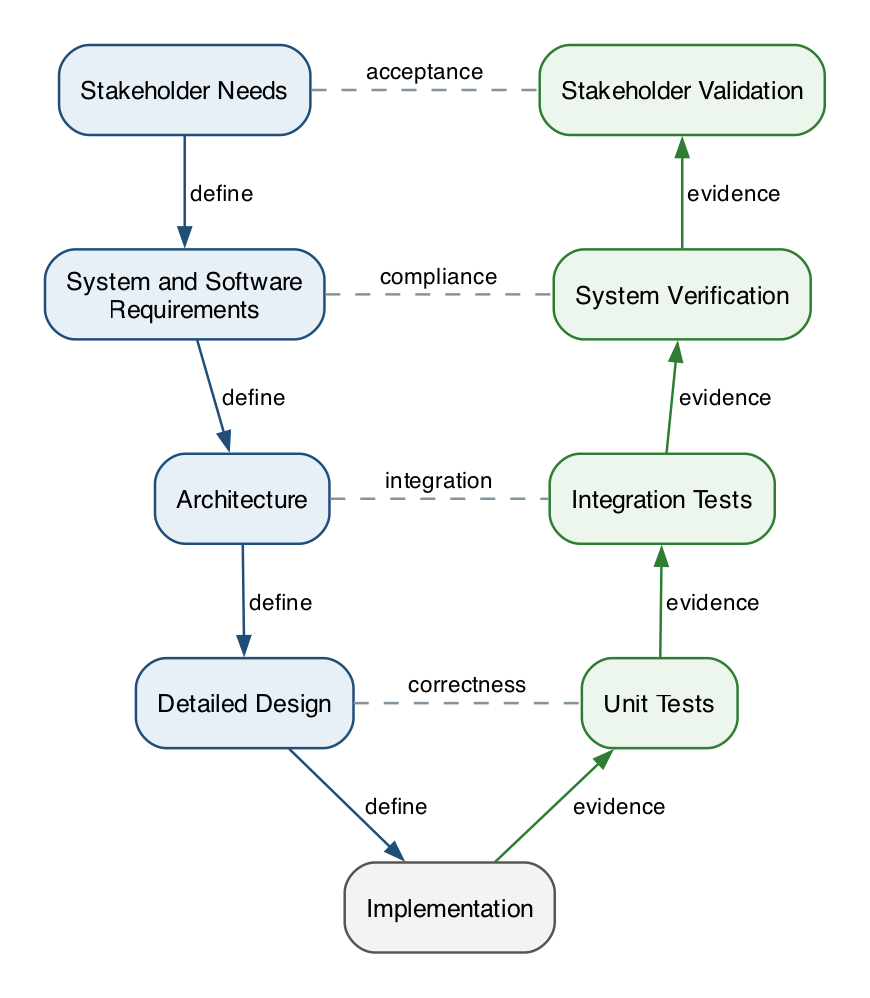
\includegraphics[width=0.92\textwidth]{png/dsnIntroduction/dsnVModel.png}
%\caption{V-model relationships used by this specification.\label{Figure:VModel}}
%\end{figure}
